\begin{figure}[H]
    \begin{center}
        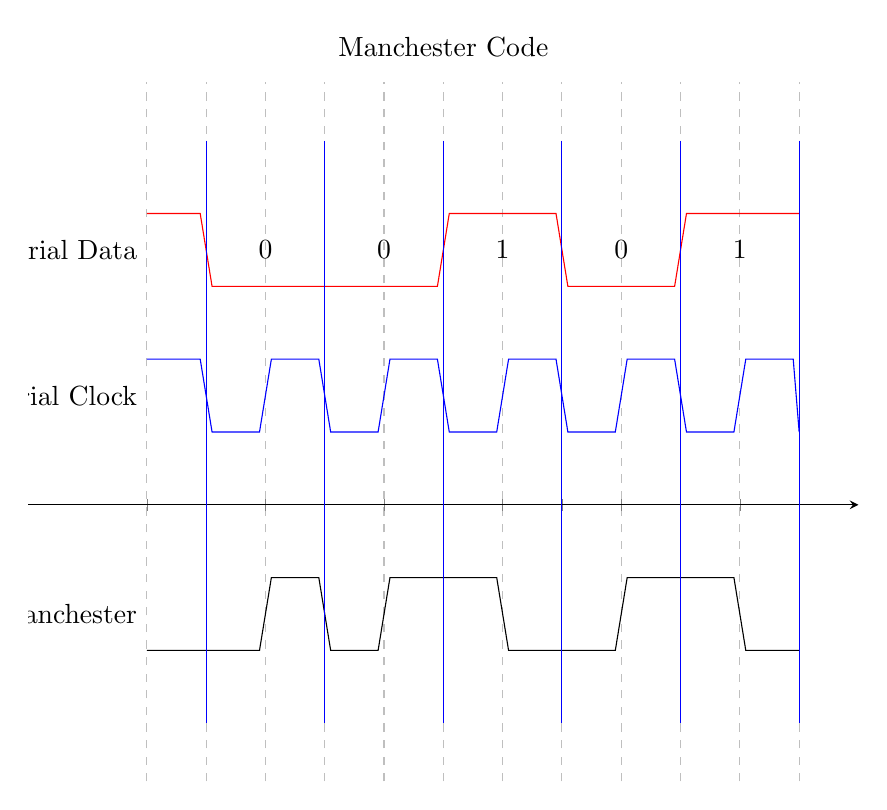
\begin{tikzpicture}
        \begin{axis} [
            width=\textwidth,
            axis x line=middle,
            axis y line=none,
            xmin=-20,
            xmax=120,
            xmajorgrids=true,
            grid style=dashed,
            xtick={0, 10, ..., 110},
            samples=1050,
            title=Manchester Code,
            xticklabels=\empty,
        ]
        
        % Serial Data
        \addplot[red] coordinates
        {(0,4) (9,4) (11,3) (49,3) (51,4) (69,4) (71,3) (89,3) (91,4) (110,4)};

        % Serial Clock
        \addplot[blue] coordinates
        {(0,2) (9,2) (11,1) (19,1) (21,2) (29,2) (31,1) (39,1) (41,2) (49,2) (51,1) (59,1) (61,2)
        (69,2) (71,1) (79,1) (81,2) (89,2) (91,1) (99, 1) (101, 2) (109,2) (110,1)};

        % Manchester
        \addplot[black] coordinates
        {(0,-2) (19,-2) (21,-1) (29,-1) (31,-2) (39,-2) (41,-1) (59,-1) (61,-2) (79,-2) (81,-1)
        (99,-1) (101,-2) (110,-2)};

        % Vertical Lines
        \addplot[blue] coordinates
        {(10,5) (10,-3)};
        \addplot[blue] coordinates
        {(30,5) (30,-3)};
        \addplot[blue] coordinates
        {(50,5) (50,-3)};
        \addplot[blue] coordinates
        {(70,5) (70,-3)};
        \addplot[blue] coordinates
        {(90,5) (90,-3)};
        \addplot[blue] coordinates
        {(110,5) (110,-3)};

        % Serial Data
        \node[] at (axis cs:20,3.5) {0};
        \node[] at (axis cs:40,3.5) {0};
        \node[] at (axis cs:60,3.5) {1};
        \node[] at (axis cs:80,3.5) {0};
        \node[] at (axis cs:100,3.5) {1};

        % Signal Labels
        \node[left] at (axis cs:0,3.5) {Serial Data};
        \node[left] at (axis cs:0,1.5) {Serial Clock};
        \node[left] at (axis cs:0,-1.5) {Manchester}; 
        \end{axis}
        \end{tikzpicture}
    \end{center}
    \caption{Manchester Code of `00101' serial data stream}
    \label{fig:manchester-code}
\end{figure}
